%! TEX root = ../000-main.tex
\section{Model complexity, VC-dimension and generalization bounds}
\index{VC-dimension}\index{complexity}\index{generalization bound}

\begin{definition}{dichotomy of a set}{dichotomy}

  Let $\mathcal{F}$ be a hypothesis set, let $S$ be a set of data points $S =
  \{x_1, \ldots, x_m\},\quad x^i \in \mathds{R}^d$.

  A \iemph{dichotomy} of a set
  $S$ is one of the possible ways of labelling the points in $S$ in
  one of two classes.

\end{definition}

\begin{definition}{Shattering}{shattering}\index{shattering}
  A set $S$ of size $m$ is said to \emph{shatter} by $\mathcal{F}$
  when all $2^m$ possible dichotomies can be realized (makes 0 TR on $S$)
  by a member of
  $\mathcal{F}$.
\end{definition}

\begin{definition}{VC-dimension}{vc-dimension-cont}
  Vapnik-Chervonenkis dimension \\[1em]
  The VC-dimension of a hypothesis space $\mathcal{F}$ is the size
  of the largest set $S$ that can be shattered by $\mathcal{F}$.
\end{definition}

\begin{example}{Intervals on the real line ($d = 1$)}{}
  \begin{equation*}
    \mathcal{F} = \{[a,\,b]\mid a < b \in \mathds{R}\}
  \end{equation*}

  The VC-dimension of $\mathcal{F}$ is $2$. With $m = 3$ points,
  we cannot shatter it. But with $m = 2$ we can:
\begin{figure}[H]
  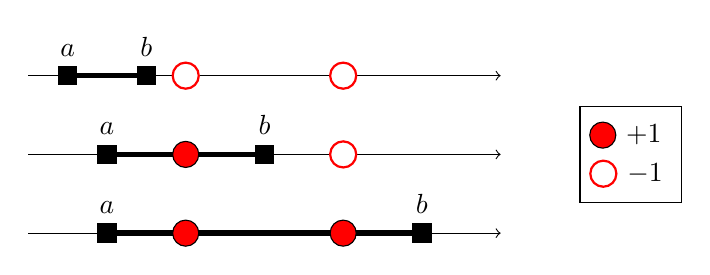
\begin{tikzpicture}[
			leftNode/.style={circle,minimum width=.5ex, fill=red,draw},
			rightNode/.style={circle,minimum width=.5ex, red, fill=white,thick,draw},
      limitNodeL/.style={draw,minimum width=0.25ex,minimum height=1ex,fill,label=$a$},
      limitNodeR/.style={draw,minimum width=0.25ex,minimum height=1ex,fill,label=$b$},
    ]

    % \addlegendimage{leftNode};
    % \addlegendentry{+1};
    % \addlegendimage{rightNode};
    % \addlegendentry{-1};

    \draw[->] (-1,0) -- (5,0);
    \draw[->] (-1,1) -- (5,1);
    \draw[->] (-1,2) -- (5,2);

    \node[limitNodeL] at (0,0) {};
    \node[limitNodeR] at (4,0) {};
    \draw[line width=2pt] (0,0) -- (4,0);
    \node[leftNode] at (1,0) {};
    \node[leftNode] at (3,0) {};

    \node[limitNodeL] at (0,1) {};
    \node[limitNodeR] at (2,1) {};
    \draw[line width=2pt] (0,1) -- (2,1);
    \node[leftNode] at (1,1) {};
    \node[rightNode] at (3,1) {};

    \node[limitNodeL] at (-0.5,2) {};
    \node[limitNodeR] at (0.5,2) {};
    \draw[line width=2pt] (-0.5,2) -- (0.5,2);
    \node[rightNode] at (1,2) {};
    \node[rightNode] at (3,2) {};

    \matrix [draw,right] at (6,1) {
      \node [leftNode,label=right:{$+1$}] {}; \\
      \node [rightNode,label=right:{$-1$}] {}; \\
    };

	\end{tikzpicture}
\end{figure}
\end{example}

\begin{example}{
  Axis aligned rectangles in $\mathds{R}^2$ ($d = 2$)
}{}
  \begin{equation*}
    \mathcal{F} = \{[a_1,\,b_1]\times [a_2,\,b_2]\mid a_1 < b_1,\, a_2 < b_2 \in \mathds{R}\}
  \end{equation*}

  The VC-dimension of $\mathcal{F}$ is $4$.

\begin{figure}[H]
  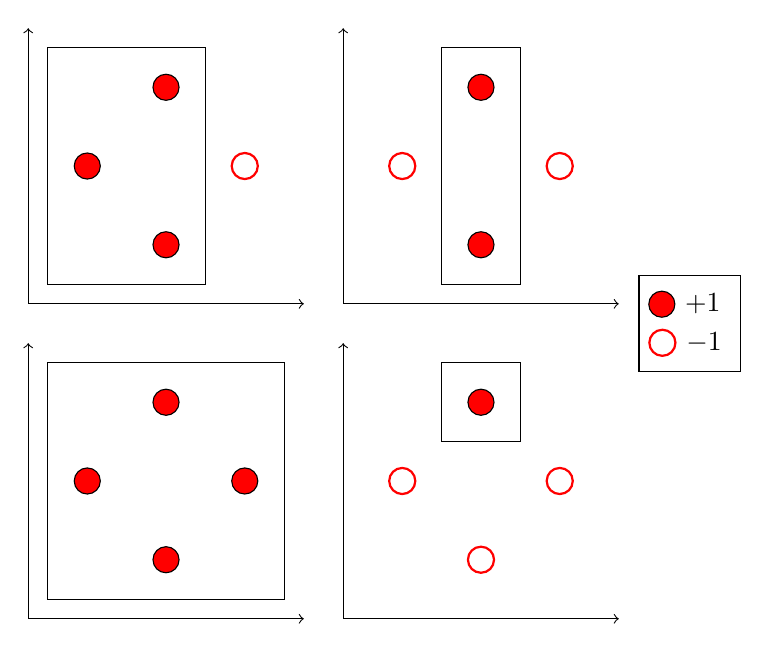
\begin{tikzpicture}[
			nodeIn/.style={circle,minimum width=.5ex, fill=red,draw},
			nodeOut/.style={circle,minimum width=.5ex, red, fill=white,thick,draw},
      limitNodeL/.style={draw,minimum width=0.25ex,minimum height=1ex,fill,label=$a$},
      limitNodeR/.style={draw,minimum width=0.25ex,minimum height=1ex,fill,label=$b$},
    ]

    \node[nodeIn] at (0, 1) {};
    \node[nodeIn] at (0, -1) {};
    \node[nodeOut] at (1, 0) {};
    \node[nodeOut] at (-1, 0) {};
    \draw (-0.5, -1.5) rectangle (0.5, 1.5);
      \draw[<->] (-1.75, 1.75) -- (-1.75, -1.75) -- (1.75, -1.75);

    \begin{scope}[shift={(-4,0)}]
      \node[nodeIn] at (0, 1) {};
      \node[nodeIn] at (0, -1) {};
      \node[nodeOut] at (1, 0) {};
      \node[nodeIn] at (-1, 0) {};
    \draw (-1.5, -1.5) rectangle (0.5, 1.5);
      \draw[<->] (-1.75, 1.75) -- (-1.75, -1.75) -- (1.75, -1.75);
    \end{scope}

    \begin{scope}[shift={(-4,-4)}]
      \node[nodeIn] at (0, 1) {};
      \node[nodeIn] at (0, -1) {};
      \node[nodeIn] at (1, 0) {};
      \node[nodeIn] at (-1, 0) {};
    \draw (-1.5, -1.5) rectangle (1.5, 1.5);
      \draw[<->] (-1.75, 1.75) -- (-1.75, -1.75) -- (1.75, -1.75);
    \end{scope}

    \begin{scope}[shift={(0,-4)}]
      \node[nodeIn] at (0, 1) {};
    \draw (-0.5, 0.5) rectangle (0.5, 1.5);
      \node[nodeOut] at (0, -1) {};
      \node[nodeOut] at (1, 0) {};
      \node[nodeOut] at (-1, 0) {};
      \draw[<->] (-1.75, 1.75) -- (-1.75, -1.75) -- (1.75, -1.75);
    \end{scope}

    \matrix [draw,right] at (2,-2) {
      \node [nodeIn,label=right:{$+1$}] {}; \\
      \node [nodeOut,label=right:{$-1$}] {}; \\
    };

	\end{tikzpicture}
  \caption{Axis aligned rectangles in $\mathds{R}^2$}
\end{figure}
\end{example}

\begin{note}
  Radamaiher complexity encompases the VC-dimension adding
  regression.
\end{note}
